% E.6 Rt△ABC, ∠ACB=90°, ∠ABC=30°, BC=6. → AC=BC·tan30°=2√3≈3.464, AB=2AC=4√3≈6.928
% C(0,0), B(6,0), A(0, 2√3). D=AC中点=(0, √3).
% P 在 AB 上(示例: P=B+0.5·(A-B)=(3, √3))
\documentclass[tikz,border=4pt]{standalone}
\usepackage{ctex}
\usepackage{amsmath}
\usetikzlibrary{calc}
\begin{document}
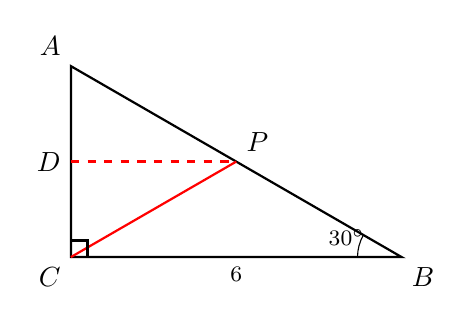
\begin{tikzpicture}[scale=0.7, thick]
  \coordinate (C) at (0,0);
  \coordinate (B) at (6,0);
  \coordinate (A) at (0,3.4641);
  \coordinate (D) at (0,1.7321);
  \coordinate (P) at (3, 1.7321);

  \draw (A)--(B)--(C)--cycle;
  \draw[red, thick] (C)--(P);
  \draw[red, thick, dashed] (D)--(P);

  % 直角 ∠C
  \draw ($(C)+(0.3,0)$)--($(C)+(0.3,0.3)$)--($(C)+(0,0.3)$);
  % 30°
  \draw[thin] (5.2,0) arc[start angle=180, end angle=150, radius=0.8];
  \node[font=\footnotesize] at (5.0, 0.35) {$30^\circ$};

  \node[below left] at (C) {$C$};
  \node[below right] at (B) {$B$};
  \node[above left] at (A) {$A$};
  \node[left] at (D) {$D$};
  \node[above right] at (P) {$P$};

  \node[below, font=\footnotesize] at ($(C)!0.5!(B)$) {$6$};
\end{tikzpicture}
\end{document}
